\section{L-TAE}
The paper ``Lightweight Temporal Self-Attention for Classifying Satellite Image Time Series" \cite{LTAE} was written by Vivien Sainte Fare Garnot and Loic Landrieu and published in 2020.

The authors present a new deep learning model for classifying satellite image time series using a modified version of the Temporal Attention Encoder.

In their proposed network, the channels of temporal inputs are distributed among several attention heads operating in parallel. These heads extract specialized temporal features, which are then concatenated into a single representation. The authors show that their approach achieves superior performance compared to other state-of-the-art time-series classification algorithms on an open-access satellite image dataset, while using significantly fewer parameters and reducing computational complexity.

Overall, the paper presents a novel method for classifying satellite image time series that utilizes a lightweight variant of temporal self-attention and outperforms other state-of-the-art approaches.

\subsection{Multi-Headed Self-Attention}

The original version of self-attention, originally developed for text translation as described in \cite{vaswani}, involves three main steps.
First, for each position $t$ in the input sequence, a key-query-value triplet is computed, denoted as $k^{(t)}$, $q^{(t)}$, and $v^{(t)}$, respectively, by applying a shared linear layer to the input $e^{(t)}$.
Second, attention masks are computed representing the compatibility (dot product) between the queries and the keys of previous elements in the sequence. 
Finally, an output is assigned to each position in the sequence, which is the sum of the previous values weighted by the corresponding attention mask.

To allow each head to specialize in detecting specific features of the feature vectors, the self-attention process is performed in parallel for $H$ sets of independent parameters or heads, and the outputs are concatenated.
This approach is used by Rußwurm et al. \cite{russwurm2019self} to embed sequences of satellite observations by max-pooling the resulting sequence of outputs in the temporal dimension.

Garnot et al. \cite{garnot2020satellite} introduce a modified self-attention scheme called the Temporal Attention Encoder (TAE).
First, they propose to use the input embeddings directly as values (i.e., $v^{(t)} = e^{(t)}$), which takes advantage of the end-to-end training of the image embedding functions along with the TAE.
They also define a single master query $\hat{q}$ for each sequence, which is computed from the temporal average of the queries.
The master query is compared to the key sequence to generate a single attention mask of dimension $T$, which is used to weight the temporal average of the values into a single feature vector.

\subsection{Model}
Their work is an extension of previous efforts to adapt multi-head self-attention for sequence embedding.
The primary goal is to optimize efficiency, especially with respect to the number of parameters and the computational load.

\begin{figure}[H]
  \centering
  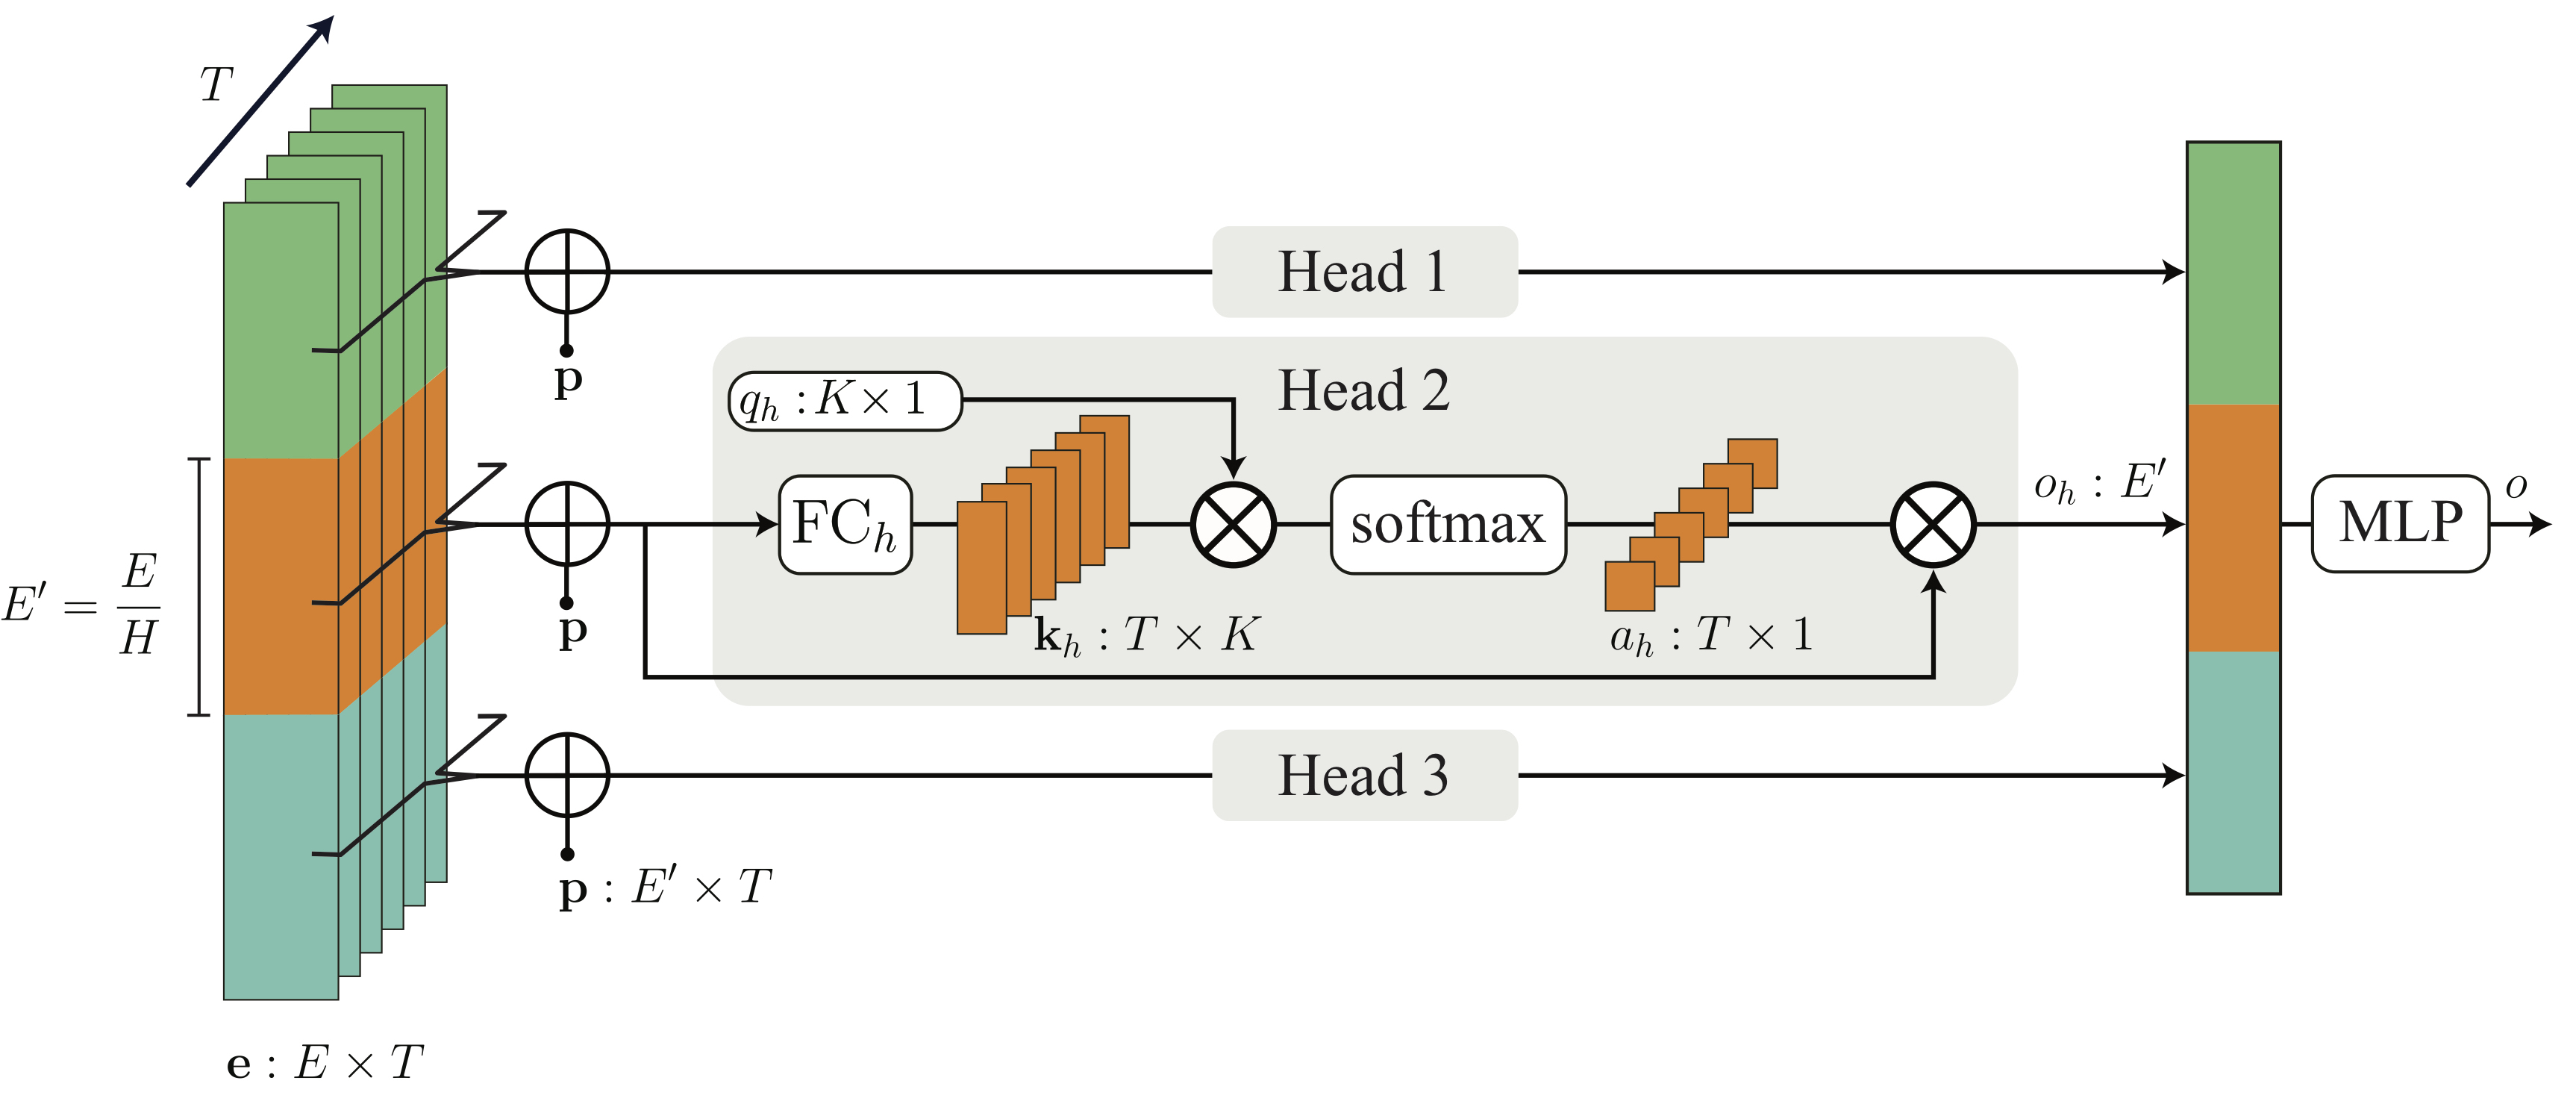
\includegraphics[width=1\textwidth]{LTAE}
  \caption{Light Temporal Attention Encoder  (L-TAE) module processing an input sequence e of $T$ vectors of
  size $E$, with $H = 3$ heads and keys of size $K$. The channels of the input embeddings
  are distributed among heads. Each head uses a learnt query $\hat{q_h}$, while a linear layer
  $FC_h$ maps inputs to keys. The outputs of all heads are concatenated into a vector with
  the same size as the input embeddings, regardless of the number of heads \cite{LTAE}}
  \label{fig:LTAErchitecture}
\end{figure}

\begin{paragraph}{Channel Grouping} 
The proposal is to divide the $E$ channels of the input elements into $H$ groups of size $E' = E/H$ following the approach of Wu et al. \cite{wu2018group}, where $H$ refers to the number of heads. The groups of input channels for the $h$-th group of the t-th element of the input sequence (\ref{eq:LTAE1}) are denoted by $e^{(t)}_h$.

To encode the number of days elapsed since the beginning of the sequence, an $E'$-dimensional positional vector $p$ with a characteristic scale $\tau = 1000$ is used (\ref{eq:LTAE2}).
To enable each head to access this information, the vector $p$ is replicated and added to every channel group.
This approach allows each head to work in parallel on its corresponding group of channels, reducing the computational expense of calculating keys and queries. Additionally, it allows each head to specialize alongside its channel group and avoid redundant operations between heads.
\end{paragraph} 

\begin{paragraph}{Query-as-Parameter} 
The K-dimensional master query $q_h$ of each head $h$ is defined as a model parameter instead of the results of a linear layer.
This approach has the immediate advantage of reducing the number of parameters required.
Although this method lacks flexibility, it is compensated by the greater number of heads available.
\end{paragraph} 

\begin{paragraph}{Attention Masks}
The approach involves using a learned linear layer (\ref{eq:LTAE3}) solely for obtaining the keys, bypassing the values $(v^{(t)} = e^{(t)})$, and employing model parameters for the queries.
For each head $h$, the attention masks $a_h \in [0, 1]^T$ are obtained by scaling the softmax of the dot product between the keys and the master query (\ref{eq:LTAE4}).
The outputs $o_h$ of each head are determined by summing the corresponding inputs weighted by the attention mask $a_h$ along the temporal dimension (\ref{eq:LTAE5}).
Following this step, the outputs of each head are concatenated to form a vector of size $E$, which is then processed through a multi-layer perceptron MLP to achieve the desired size (\ref{eq:LTAE6}).

A schematic representation of the network is provided in Figure \ref{fig:LTAErchitecture}.
In summary, the various steps of the L-TAE method can be summarized by the following operations for $h = 1...H$ and $t = 1...T$:

\begin{align}
  e^{(t)}_h &= e^{(t)}[(h-1) E'...hE']                                  \label{eq:LTAE1}\\
  [p^{(t)}] &= sin(day(t)/\tau^{\frac{i}{E'}})                          \label{eq:LTAE2}\\
  k^{(t)}_h &= FC_h(e^{(t)}_h + p^{(t)})                                \label{eq:LTAE3}\\
  a_h       &= softmax \Bigr(\frac{1}{\sqrt{K}} \Bigr[[q_h \cdot k^{(t)}_h\Bigr]^T_{t=1}\Bigr) \label{eq:LTAE4}\\
  o_h       &= \sum_{t=1}^{T} a_h[t] (e^{(t)}_h + p^{(t)})              \label{eq:LTAE5}\\
  o         &= MLP([o_1,...,o_H]).                                      \label{eq:LTAE6}
\end{align}

\end{paragraph}

\begin{paragraph}{Spatio-temporal classifier}
The L-TAE temporal encoder is designed to be trained together with a spatial encoding module and a decoder module in an end-to-end manner (\ref{eq:LTAE7}).
  
The spatial encoder $S$ is responsible for mapping a sequence of raw inputs $X^{(t)}$ to a sequence of learned features $e^{(t)}$, computed independently at each position of the sequence.
On the other hand, the decoder $D$ is responsible for mapping the output $o$ of the L-TAE to a target vector $y$, which can be class logits in the case of a classification task.
\end{paragraph}

\begin{equation}
  \label{eq:LTAE7}
  \Bigr[X^{(t)}\Bigr]^T_{t=1} \quad \xrightarrow{S} \quad \Bigr[e^{(t)}\Bigr]^T_{t=1} \quad \xrightarrow{L\mbox{--}TAE} \quad o \quad \xrightarrow{D} \quad y
\end{equation}